%%========================================================================
%% LaTeX sjabloon voor stage/projectrapport of bachelorproef
%%  HoGent Bedrijf en Organisatie
%%========================================================================

%%========================================================================
%% Preamble
%%========================================================================

\documentclass[pdftex,a4paper,12pt,twoside]{report}

% XXX: Let op: dit sjabloon is gemaakt om dubbelzijdig af te drukken
% Voor enkelzijdig, verwijder ``twoside'' hierboven.

%%---------- Extra functionaliteit ---------------------------------------

\usepackage[utf8]{inputenc}  % Accenten gebruiken in tekst (vb. é ipv \'e)
\usepackage{amsfonts}        % AMS math packages: extra wiskundige
\usepackage{amsmath}         %   symbolen (o.a. getallen-
\usepackage{amssymb}         %   verzamelingen N, R, Z, Q, etc.)
\usepackage[dutch]{babel}    % Taalinstellingen: woordsplitsingen,
                             %  commando's voor speciale karakters
                             %  ("dutch" voor NL)
\usepackage{eurosym}         % Euro-symbool €
\usepackage{geometry}
\usepackage{graphicx}        % Invoegen van tekeningen
\usepackage[pdftex,bookmarks=true]{hyperref}
                             % PDF krijgt klikbare links & verwijzingen,
                             %  inhoudstafel
\usepackage{listings}        % Broncode mooi opmaken
\usepackage{multirow}        % Tekst over verschillende cellen in tabellen
\usepackage{rotating}        % Tabellen en figuren roteren
\usepackage{natbib}          % Betere bibliografiestijlen
\usepackage{fancyhdr}        % Pagina-opmaak met hoofd- en voettekst

\usepackage[T1]{fontenc}     % Ivm lettertypes
\usepackage{lmodern}
\usepackage{textcomp}

\usepackage{lipsum}          % Voor vultekst (lorem ipsum)
\usepackage[section]{placeins}
\usepackage{float}
%%---------- Layout ------------------------------------------------------

% hoofdingen, enz.
\pagestyle{fancy}
% enkel hoofdstuktitel in hoofding, geen sectietitel (vermijd overlap)
\renewcommand{\sectionmark}[1]{}

% lijn, wordt gebruikt in titelpagina
\newcommand{\HRule}{\rule{\linewidth}{0.5mm}}

% Leeg blad
\newcommand{\emptypage}{
\newpage
\thispagestyle{empty}
\mbox{}
\newpage
}

% Gebruik een schreefloos lettertype ipv het "oubollig" uitziende
% Computer Modern
\renewcommand{\familydefault}{\sfdefault}

% Commando voor invoegen Java-broncodebestanden (dank aan Niels Corneille)
% Gebruik: \codefragment{source/MijnKlasse.java}{Uitleg bij de code}
\newcommand{\codefragment}[2]{ \lstset{%
  language=java,
  breaklines=true,
  float=th,
  caption={#2},
  basicstyle=\scriptsize,
  frame=single,
  extendedchars=\true
}
\lstinputlisting{#1}}

%%---------- Documenteigenschappen ---------------------------------------
%% Vul dit aan met je eigen info:

% Je eigen naam
\newcommand{\student}{Gianni Stubbe}

% De naam van je lector, begeleider, promotor
\newcommand{\promotor}{Jens Buysse}

% De naam van je co-promotor
\newcommand{\copromotor}{Bert Van Vreckem}

% Indien je bachelorproef in opdracht van een bedrijf of organisatie
% geschreven is, geef je hier de naam.
\newcommand{\instelling}{}

% De titel van het rapport/bachelorproef
\newcommand{\titel}{Automatische opzet van Cisco netwerkapparatuur in combinatie met Ansible}

% Datum van indienen
\newcommand{\datum}{26 augustus 2016}

% Faculteit
\newcommand{\faculteit}{Faculteit Bedrijf en Organisatie}

% Soort rapport
\newcommand{\rapporttype}{Scriptie voorgedragen tot het bekomen van de graad van\\Bachelor in de toegepaste informatica}

% Academiejaar
\newcommand{\academiejaar}{2015-2016}

% Examenperiode
%  - 1e semester = 1e examenperiode
%  - 2e semester = 2e examenperiode
%  - tweede zit = 3e examenperiode
\newcommand{\examenperiode}{Derde examenperiode}

%%========================================================================
%% Inhoud document
%%========================================================================

\begin{document}

%%---------- Front matter ------------------------------------------------
%% Het voorblad - Hier moet je in principe niets wijzigen.

\begin{titlepage}
  \newgeometry{top=2cm,bottom=1.5cm,left=1.5cm,right=1.5cm}
  \begin{center}

    \begingroup
    \rmfamily
    
\includegraphics[width=2.5cm]{img/HG-beeldmerk-woordmerk}\\[.5cm]
    \faculteit\\[3cm]
    \titel
    \vfill
    \student\\[3.5cm]
    \rapporttype\\[2cm]
    Promotor:\\
    \promotor\\
    Co-promotor:\\
    \copromotor\\[2.5cm]
    Instelling: \instelling\\[.5cm]
    Academiejaar: \academiejaar\\[.5cm]
    \examenperiode
    \endgroup

  \end{center}
  \restoregeometry
\end{titlepage}

% Schutblad

\emptypage


\begin{titlepage}
  \newgeometry{top=5.35cm,bottom=1.5cm,left=1.5cm,right=1.5cm}
  \begin{center}

    \begingroup
    \rmfamily
    \faculteit\\[3cm]
    \titel
    \vfill
    \student\\[3.5cm]
    \rapporttype\\[2cm]
    Promotor:\\
    \promotor\\
    Co-promotor:\\
    \copromotor\\[2.5cm]
    Instelling: \instelling\\[.5cm]
    Academiejaar: \academiejaar\\[.5cm]
    \examenperiode
    \endgroup

  \end{center}
  \restoregeometry
\end{titlepage}


\begin{abstract}
%% TODO: De "abstract" of samenvatting is een kernachtige (~ 1 blz. voor een
%% thesis) synthese van het document.
%%
%% Deze aspecten moeten zeker aan bod komen:
%% - Context: waarom is dit werk belangrijk?
%% - Nood: waarom moest dit onderzocht worden?
%% - Taak: wat heb je precies gedaan?
%% - Object: wat staat in dit document geschreven?
%% - Resultaat: wat was het resultaat?
%% - Conclusie: wat is/zijn de belangrijkste conclusie(s)?
%% - Perspectief: blijven er nog vragen open die in de toekomst nog kunnen
%%    onderzocht worden? Wat is een mogelijk vervolg voor jouw onderzoek?
%%
%% LET OP! Een samenvatting is GEEN voorwoord!

Internet is tegenwoordig niet meer weg te denken maar om het op te zetten is er vaak toch heel wat werk voor nodig voor een netwerkbeheerder. Zeker bij grotere bedrijven kan het configureren een tijdrovende taak zijn die vaak heel repetitief en gelijkaardig is. De laatste jaren is er veel vooruitgang geboekt bij het automatiseren van servers met behulp van verschillende frameworks en tools. Het volgende onderdeel die aan de beurt is zijn verschillende componenten uit het netwerksegment zoals switches, routers en wifi-controllers. 
\\

Meer specifiek zal er geconcentreerd worden op het automatiseren met de Ansible architectuur. Deze is uitgebreid in de les gezien bij Meneer Van Vreckem en ook in het werkveld kom je dit al maar vaker tegen. Het zou dus interessant zijn om netwerkapparatuur automatisch te kunnen configureren met dezelfde kennis die de systeembeheerders al hebben. 
\\

In het document ga ik even onderzoek doen naar bestaande automatisatie methoden en waarom er voor Ansible gekozen is naast het gezien te hebben in de lessen. Daarna zal er een basis configuratie gemaakt worden met Cisco apparatuur bestaande uit 1 router en 2 switches. Deze wordt getest en de criteria die moeten voldoen worden genoteerd. Hierna wordt een "Playbook" gemaakt in Ansible en wordt deze toegepast op de apparatuur. Deze zal aan de hand van vooropgestelde resultaten vergeleken worden met de nieuwe resultaten behaald met Ansible. 

%% TODO: BESCHRIJVEND VAN RESULTATEN
  
\end{abstract}

\chapter*{Voorwoord}
\label{ch:voorwoord}

%% TODO:
%% Het voorwoord is het enige deel van de bachelorproef waar je vanuit je
%% eigen standpunt (``ik-vorm'') mag schrijven. Je kan hier bv. motiveren
%% waarom jij het onderwerp wil bespreken.
%% Vergeet ook niet te bedanken wie je geholpen/gesteund/... heeft


\tableofcontents

% Als je een lijst van afkortingen of termen wil toevoegen, dan hoort die
% hier thuis. Gebruik bijvoorbeeld de ``glossaries'' package.

%%---------- Kern --------------------------------------------------------

\chapter{Inleiding}
\label{ch:inleiding}

De bachelorproef speelt zich af binnen de eSports scene. eSports staat voor ''electronic sports'' \citep{BenDirs2015}. Dit is een overkoepelende term voor alles dat met competitief gamen te maken heeft. Het kan vrij letterlijk gezien worden als een sport maar dan achter een computerscherm. Net als gewone professionele sporters hebben eSporters een strak trainingsschema die tot wel meer dan 12u per dag tijd in neemt. Wanneer er toernooien gespeeld worden valt er voor de spelers tot wel 18 miljoen dollar aan prijzengeld te winnen. \citep{dota2theinternational} 
\\

Wat eSports ook zo kenmerkend maakt is dat het vrij nieuw is maar toch al heel veel mensen aantrekt. Het platform bij uitstek om eSports te volgen is ''Twitch.tv'', hiermee kunnen mensen matchen, toernooien maar ook individuen bekijken die aan het gamen zijn. Op bepaalde momenten kunnen er tot wel enkele miljoenen mensen gelijktijdig kijken naar de grootste competities ter wereld op het vlak van gaming. Gemiddeld zijn er 500.000 mensen aan het kijken naar wat er zoal gespeeld wordt door andere mensen voor een totaal van 241.441.823.059 minuten over het jaar 2015. \citep{twitchinfographic}
\begin{figure}[!h]
\centering
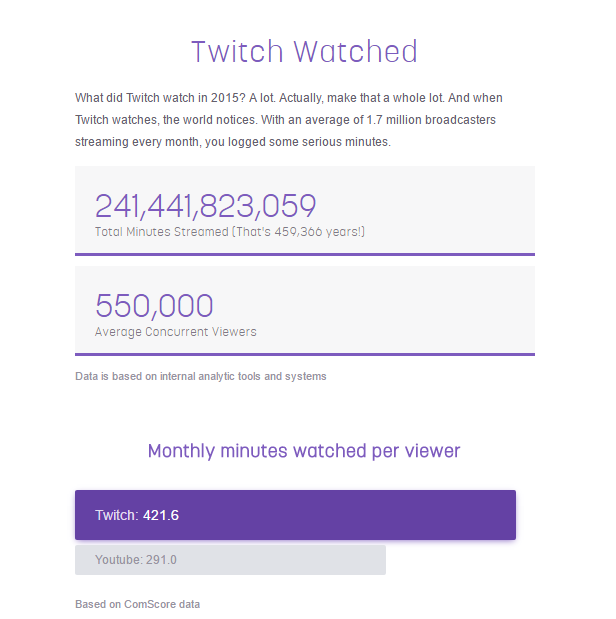
\includegraphics[width=15cm]{img/TwitchInfographic}
\caption{Aantal uren bekeken beelden op Twitch.tv}
\end{figure}  
\\

Het genre game waar deze thesis zich op zal specialiseren zijn ''FPS games''. Dit staat voor First Person Shooters of met andere woorden, games waarbij mensen zich in een bepaald personage wagen en uit het standpunt van die persoon kijken. De grootste game die momenteel competitief gespeeld wordt in de eSports scene (onder de categorie FPS Games) is de alom bekende Counter-Strike: Global Offensive. 
 Met een 10 miljoen unieke spelers per maand heeft dit spel een heel grote spelersbasis en spelers van overal ter wereld. Dit is een van de meest bekeken games op Twitch en is ook een van de eenvoudigste games om te snappen vergeleken met de andere populaire eSports games. \citep{csgoblog}
\\

Het nadeel aan deze game is het grote aantal valsspelers of ''cheaters''. Veel spelers zijn snel geneigd om een van de veelvuldige cheats te downloaden en deze even te proberen wanneer ze een minder moment hebben. Het is dan ook helemaal niet moeilijk om deze te vinden na wat zoeken op het internet. Na even zoeken komen we de volgende voorbeelden al tegen:

 Mensen downloaden deze dan even naar hen pc en schakelen deze dan in om voordelen te krijgen op het vlak van ''aim'' - het mikken met een geweer - of op vlak van ''pressence'' - mensen zien terwijl deze zich achter een muur bevinden (ook wel wallhack genoemd). Daarna gaat dit nog veel verder tot zelf de kleinste dingen zoals het rondspringen waardoor je meer snelheid haalt - bunnyhoppen genaamd -, dit is normaal gezien iets wat heel veel oefening bevat en zelf de beste spelers niet consistent kunnen doen. 
\\

Voor dit onderzoek zal er vooral geconcentreerd worden op het spel Counter-Strike omdat dit het meest gekend is en er dus ook het diepst op ingegaan kan worden. De technieken om vals te spelen en dit tegen te gaan zijn vrij gelijklopend tussen verschillende FPS games zoals Counter-Strike, Battlefield, Call of Duty,... De technieken die hier dan ook toegepast worden zullen parallel lopen voor deze voorgenoemde andere games.
\\

Eerst wordt er ieder aspect uitgelegd van wat nodig is te weten om het spel te snappen. Daarna zullen we de veelvuldige valsspeel manieren en tools om dit tegen te gaan bekijken.


\section{Probleemstelling en Onderzoeksvragen}
\label{sec:onderzoeksvragen}
% TODO: Wees zo concreet mogelijk bij het formuleren van je
% onderzoeksvra(a)g(en). Een onderzoeksvraag is trouwens iets waar nog
% niemand op dit moment een antwoord heeft (voor zover je kan nagaan).

Voor dit onderzoek gaan we dus op zoek naar een oplossing om cheaters tegen te gaan binnen FPS games toegepast op Counter-Strike. Dit met de bedoeling om op een online platform te implementeren zodat competities binnen games zo eerlijk mogelijk kunnen verlopen. Wat is de beste en meest praktische oplossing voor deze use case. 
\\

Waarom is het zo moeilijk om dit tegen te gaan en valt er iets te doen naast anti-cheating om dit tegen te gaan.


\chapter{Methodologie}
\label{ch:methodologie}

% TODO: Hoe ben je te werk gegaan? Verdeel je onderzoek in grote fasen, en
% licht in elke fase toe welke stappen je gevolgd hebt. Verantwoord waarom je
% op deze manier te werk gegaan bent. Je moet kunnen aantonen dat je de best
% mogelijke manier toegepast hebt om een antwoord te vinden op de
% onderzoeksvraag.

In dit onderzoek ga ik eerst de lezer uitleggen wat de game Counter-Strike precies inhoudt. Het is moeilijk om ieder aspect van het onderzoek te snappen zonder dat de basis van het spel duidelijk is. Hierna wordt er eerst dieper ingegegaan op de verschillende soorten cheats en wat meer over de werking hiervan. Vervolgens wordt er gekeken welke precieze manieren er zijn om dit tegen te gaan. Dit is opgedeeld in 2 hoofdcategorieën: eerst de softwaretools die vaak beter gekend zijn, daarna wat meer over een nieuwe oplossing met hardware. 
\\

Als laatste is het de bedoeling om een testopstelling te maken die op de servers test welke cheats gevangen worden door welke anti-cheats. Er wordt dan gekeken welke opties de beste oplossing biedt en of er een combinatie mogelijk is om zo veel mogelijk valsspelers tegen te gaan. 


\chapter{Counter-Strike: Global Offensive}
\label{ch:csgo}
Voor we beginnnen aan het onderzoek naar verschillende manieren om vals te spelen en om deze tegen te gaan moeten we eerst de basis van het spel snappen. In dit onderzoek gaat het om het spel Counter-Strike: Global Offensive of kort ''CSGO''. Deze game is een van de meest gespeelde competitieve games en staat er voor gekend om eenvoudig aan te leren zijn vergeleken met andere competitieve eSports games. 
\\

De voorganger van deze immens populaire game werd uitgebracht op 19 juni 1999. Origineel was dit een modificatie voor de uiteengezette en beruchte game "Half-Life". Veel games die vandaag de dag als alleenstaande verkocht worden zijn ooit begonnen als een speltype gemaakt door spelers die bouwden op de basis van Half-Life. Na deze mod heeft Valve (de huidige ontwikkelaar achter Counter-Strike en Half-Life) een samenwerking met deze spelers aangekondigd en kon de game als alleenstaand spel gespeeld worden.
\\

Na vele beta's en heel wat patches werd de final versie gereleased. Deze release is een van de bekendste bij het competitieve onderdeel van Counter-Strike, deze staat gekend als "1.6". Dit werd snel een van de meest populaire competitieve computer games ooit en werd tot voor kort nog altijd gespeeld door veel professionele gamers hoewel deze toch al wat leeftijd had.
\citep{dusttodust}
\\

Hierna kwamen nog een andere versie genaamd ''Counter-Strike: Source''. Hoewel deze ook heel wat verkoop had is deze minder gespeeld geweest. De game waar wij ons op zullen concentreren is de in 2012 geïntroduceerde ''Counter-Strike: Global Offensive''. Deze versie van het spel is deze die vandaag de dag nog altijd gebruikt wordt.

\section{Algemeen doel van het spel}
\label{sec:algemeen doel van het spel}
Counter-Strike is niet zoals de meeste andere FPS games. Waar bij vele shooter games het vooral gaat om het gewoon neerschieten van de tegenstander en het aantal ''kills'' of ''deaths'' telt is dit bij Counter-Strike toch nog goed anders.
\\

Bij Counter-Strike spelen er vijf spelers in twee teams, deze teams kunnen ofwel ''Counter-Terrorist'' (of CT) ofwel ''Terrorist'' (of T) zijn. Elk team heeft zijn eigen doel doorheen het spel. Heel eenvoudig kunnen we zeggen dat de Terrorists als doel hebben ofwel de ene bom die ze hebben tot ontploffing te brengen, ofwel door alle Counter-Terrorists te doden. 
De Counter-Terrorists daarentegen hebben dan als doel ofwel de bom onschadelijk te maken (als deze geplaatst werd) of om alle Terrorists te doden. Dit wordt herhaald tot een maximaal van 30 ronden die elk een 2 tal minuten duren. Aan 15 ronden (of halverwege het spel) worden de teams omgewisseld van kant, de Counter-Terrorists worden dan de Terrorist en omgekeerd. Het eerste team dat 16 ronden wint in totaal wordt de winnaar van de game gezien.
\\

Een game wordt gespeeld op een bepaalde ''map'' of kaart. Deze bevat een locatie waar de Terrorist bij het begin van de ronde starten -Terrorists spawn- en een waar de CT's spawnen. Naast dit zijn er nog 2 locaties waar de bom geplaatst kan worden per kaart, dit zijnde: Bomb site A en Bomb site B. Daar kunnen ze binnen een bepaald afgebakend gebied de bom plaatsen om daarna de komst van de CT's af te wachten. Iedere map heeft ook unieke eigenschappen en maakt het daardoor vaak iets voordeliger om te starten aan een specifieke kant.
\\

Dit klinkt nog allemaal niet zo moeilijk tot nu toe maar buiten deze regels heb je nog het geld die iedere speler heeft. Ieder team begint de eerste ronde met \$800 en kan daarmee kiezen om iets te kopen van wapen of iets van ''utility'' of ''gear'' zoals een ''defuse kit'' (hiermee kan wordt de tijd voor het onschadelijk maken van de bom gehalveerd) of een kevlar vest waardoor je minder schade krijgt. 
Omdat er in de eerste ronde niet veel geld ter beschikking staat kan er niet anders gekocht worden dan een pistool en wordt deze ronde ook wel de ''pistol round'' genoemd.
\\

Iedere ronde krijgt een bepaalde speler geld voor zichzelf of voor het team aan de hand van wat er gedaan wordt. Voor een kill met een specifiek wapen komt er een bedrag bij de speler zijn pot. Hetzelfde voor het plaatsen van de bom. Maar als de bom tot onploffing gebracht wordt krijgt het hele team geld. Het verliezende team krijgt dit dan ook maar een heel stuk minder.
\\

Dit is een van de belangrijkste aspecten van het spel, het is heel handig als je kan inschatten of het ander team alles kan kopen die nodig is of als deze zullen moeten sparen en dan de ronde erna alles zullen kopen. Het sparen en enkel spelen met het standaard pistool wordt ook wel ''eco'' genoemd. Als je als een van de laatste spelers overblijft in je team en het ander team heeft nog alle spelers in leven zal het wapen vaak gespaard worden voor de volgende ronde, dit noemt men ook wel eens ''saven''.

%% TODO: de structuur en titel van deze hoofdstukken hangen af van je
% eigen onderzoek. Elke fase in je onderzoek kan een eigen hoofdstuk krijgen. Kies telkens een gepaste titel. ``Corpus'' is *GEEN* gepaste titel

\chapter{Cheats}
\label{ch:cheats}

Om te snappen hoe we het valsspelen moeten tegengaan moeten we eerst begrijpen hoe het valsspelen precies werkt. Er wordt een korte introductie gemaakt bij iedere soort en wat ze precies doen. Verder wordt er uitgelegd waarom ze precies zo vervelend zijn.
\\

De taal waarin vele cheats geschreven zijn is Assembly. Dit is een heel low level language. Dit gaat dus vaak inspelen op memory adresses en in direct contact met de CPU van een computer. Het nadeel aan deze taal is dat er vaak geen mogelijkheden die andere programmeertalen zo interessant maken zoals variabelen, overerving...
\citep{assembly}

\section{Soorten}
\label{sec:soorten}
\section{Wallhacks}
\label{sec:walls}
De eerste onderscheiding die we maken zijn ''wallhacks''. Dit is een van de meest gebruikte termen onder spelers. Vaak wordt er mis melding gemaakt van deze cheats omdat ze het meest gekend zijn. Maar wat is het nu precies?
\\

Als je je in het spel begeeft kun je met wallhacks heel eenvoudig iedereen zien lopen door de muur. Dit kan op verschillende manieren weergegeven worden. De eenvoudigste methode die door programmeurs gebruikt wordt is de box methode. Deze tekent rond ieder persoon een hokje die je door alle objecten in het spel kan zien. Zo kan je anticiperen waar de vijand zal verschijnen en heb je dus teveel oneerlijke informatie. 
De tweed manier die iets duidelijker te zien valt is met een outline rond de persoon die de vorm weergeeft hoe deze precies staat. Dit maakt het nog iets eenvoudiger voor de valsspeler omdat deze ook perfect weet waar de persoon zijn hoofd is, zijn armen enz. Op die manier kan je dus heel eenvoudig al op iemand zijn hoofd gaan mikken. Ook kan de visibiliteit erg verbeteren waardoor je wederom het onfair voordeel haalt.

Hieronder even de 2 verschillen naast elkaar.

\begin{figure}[H]
\centering
\begin{minipage}{0.48\textwidth}
\centering
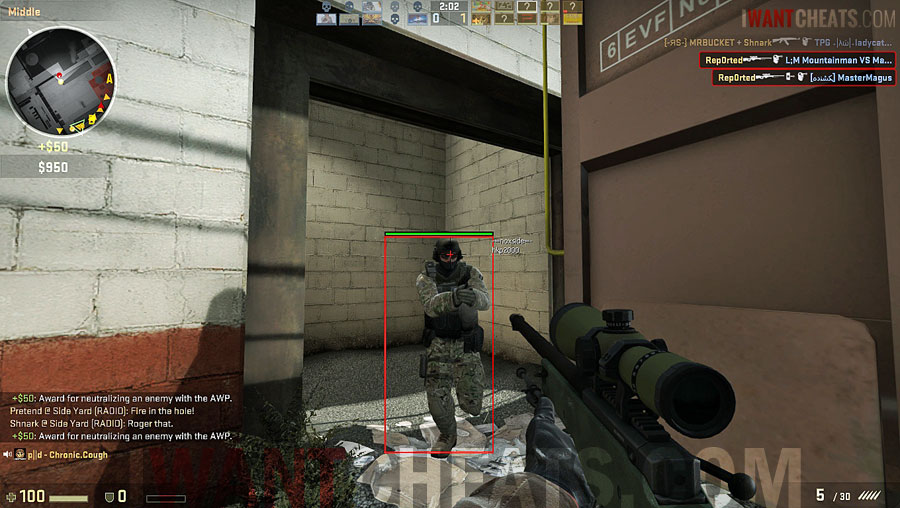
\includegraphics[width=7cm]{img/wallhack-example-box}
\caption{Wallhack met een box (merk het rode hokje op rond de persoon)}
\end{minipage}\hfill
\begin{minipage}{0.48\textwidth}
\centering
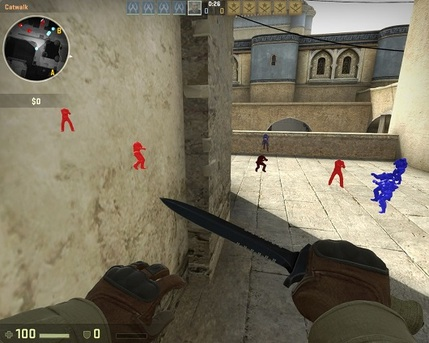
\includegraphics[width=7cm]{img/wallhack-example-outline}
\caption{wallhack met outline}
\end{minipage}
\end{figure}  

Een persoon met deze extra informatie kan op veel verschillende manier het spel beïnvloeden. Een van de eerste manieren om dit te doen is gewoon letterlijk volgen waar het andere team heengaat en anticiperen op deze situatie. Dit kan dan ook bijvoorbeeld meegedeeld worden aan een teammaat die niet aan het valsspelen is. Zo kan je als enige cheater heel eenvoudig het volledige spel beïnvloeden.

%(http://www.theregister.co.uk/2001/05/10/asus_releases_games_cheat_drivers/)

\subsection{Werking}
\label{subsec:werking}
Hoe is het precies mogelijk dat mensen weergegeven worden door de muur? Dat heeft te maken met de pakketten die tussen server en client worden verzonden. Iedere server verzend zijn pakketten naar de client, dit bevat de data van waar je teammates rondlopen, waar de vijand rondloopt, waar er smokes liggen en waar schoten geregistreerd zijn. De client zend zelf door wat er precies gebeurd achter de speler zijn pc. Dit zijn: waar die precies rondloopt, wanneer hij schiet en waar, welk wapen deze gebruikt en andere. Hoe de meeste gameservers werken is als volgt: alle data wordt doorgestuurd naar de client waar de onderdelen verwerkt worden. Dus de locatie van de niet zichtbare vijanden worden verzonden naar de client maar deze beslist wanneer deze weer te geven en wanneer niet.
\\

Voor cheatontwikkelaars is het dus zo dat zij de data die de server verzend - maar normaal niet wordt weergegeven door de client - via hun software toch wordt weergegeven. Dit dan op de verschillende manieren zoals hierboven weergegeven.
\\

Dit in Counter-Strike recent tegengegaan door de data die verzonden wordt door de server te minimaliseren. Enkel echt relevante data wordt doorgestuurd naar de client. Dus veel wallhacks werken hierdoor niet meer omdat niet alle data bij de gebruiker aanwezig is. De naam van de technologie hierachter is PVS of ''Potentially Visible Set''. Dit berekent wanneer een gebruiker een vijand kan zien en of horen en aan de hand daarvan wordt de data doorgestuurd. Op die manier is het enkel mogelijk voor cheats om personen weer te geven als deze ofwel door een teammaat gezien werden of wanneer je ze zelf ziet. Dit bestond al een heel stuk langer om de game te optimaliseren door te berekenen vanaf welke plaats je welke objecten kan zien maar nu wordt dit dus ook gedaan met de spelers zelf. 
\citep{PVS}

\section{ESP}
\label{ESP}
Als tweede cheat hebben we ESP wat staat voor ''Extrasensory Perception''. Extrasensory perception komt uit de wereld van de telepathie, wat gedefiniëerd kan worden als "the ability to know things (such as what another person is thinking or what will happen in the future) that cannot be known by normal use of the senses" \citep{extrasensoryperception}. We vermelden deze als tweede omdat ESP heel vaak wordt gebruikt in combinate met wallhacks. Net zoals bij de telepathie geeft deze extra hulp aan de gebruiker door informatie door te geven over de vijand. Dit niet over de locatie waar deze loopt maar vaak eerder over hoeveel geld de vijand beschikt en hoeveel health een bepaalde vijand nog heeft.
Omdat dit heel 'droge' informatie is wordt dit vaak weergegeven naast een wallhack. Een voorbeeld kan je hieronder zien, let vooral duidelijk op het groene lijntje erbij. Dit is hoeveel levenspunten of ''health'' de vijand nog over heeft.
\begin{figure}[!hb]
\centering
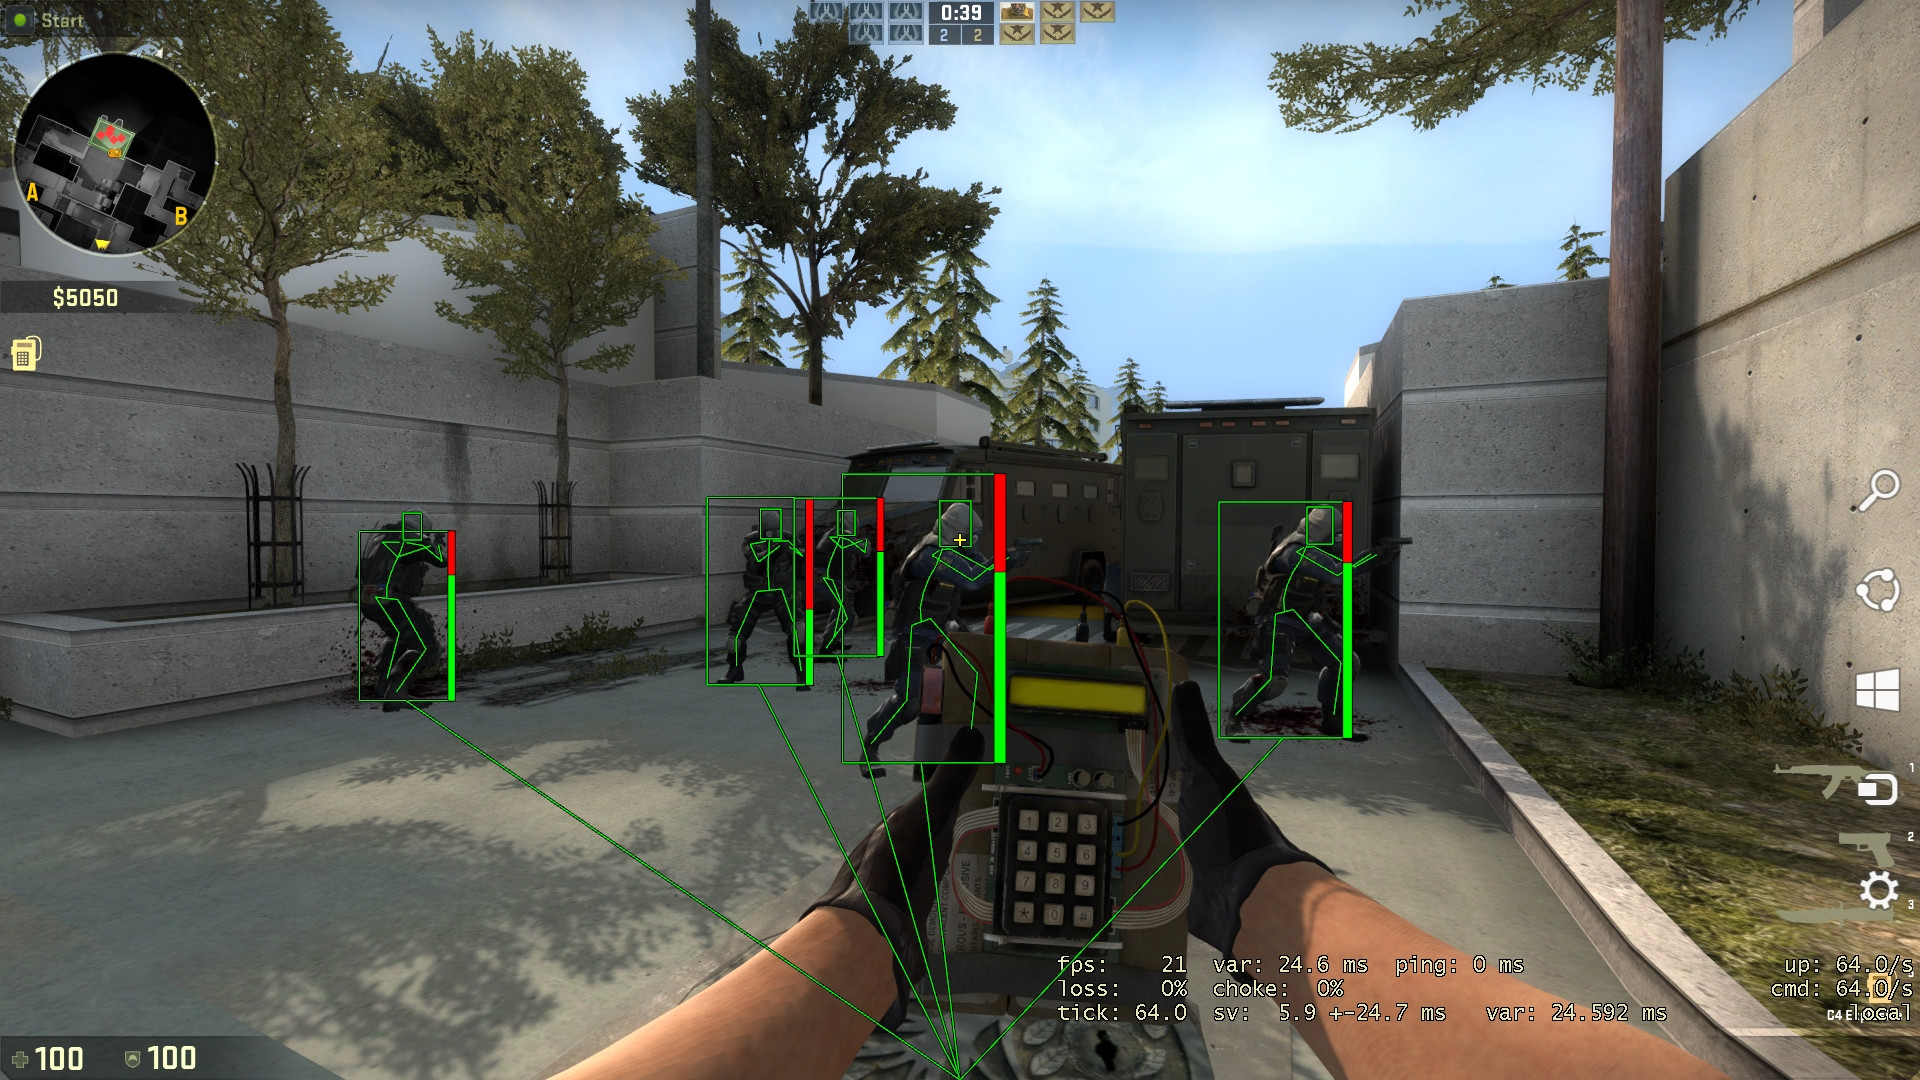
\includegraphics[width=15cm]{img/esp-example}
\caption{Wallhack in combinatie met ESP (let op het groene balkje die aanduidt hoeveel leven nog resterend is per persoon)}
\end{figure}
  
\section{Aimhacks}
\label{sec:aim}
Wat het spel Counter-Strike nu zoveel anders maakt vergeleken met andere FPS-games is dat deze heel wat training vereist om ieder wapen te kunnen beheersen. Het is zo dat ieder wapen een bepaald uniek karakter heeft. Bij gewone geweren of ''Rifles'' is er vaak een patroon die deze volgt als je hem in 1 keer leegschiet, dit wordt het ''spray pattern'' genoemd. Dit is het omhoog gaan van het wapen in een bepaalde beweging wanneer je schiet. Omdat dit altijd hetzelfde is kan je ook dit tegengaan door je muis in de tegengestelde richting naar beneden en/of naar linkgs of rechts te bewegen. Een voorbeel van zo'n spray pattern is hieronder afgebeeld voor een van de wapens.

\begin{figure}[!hb]
\centering
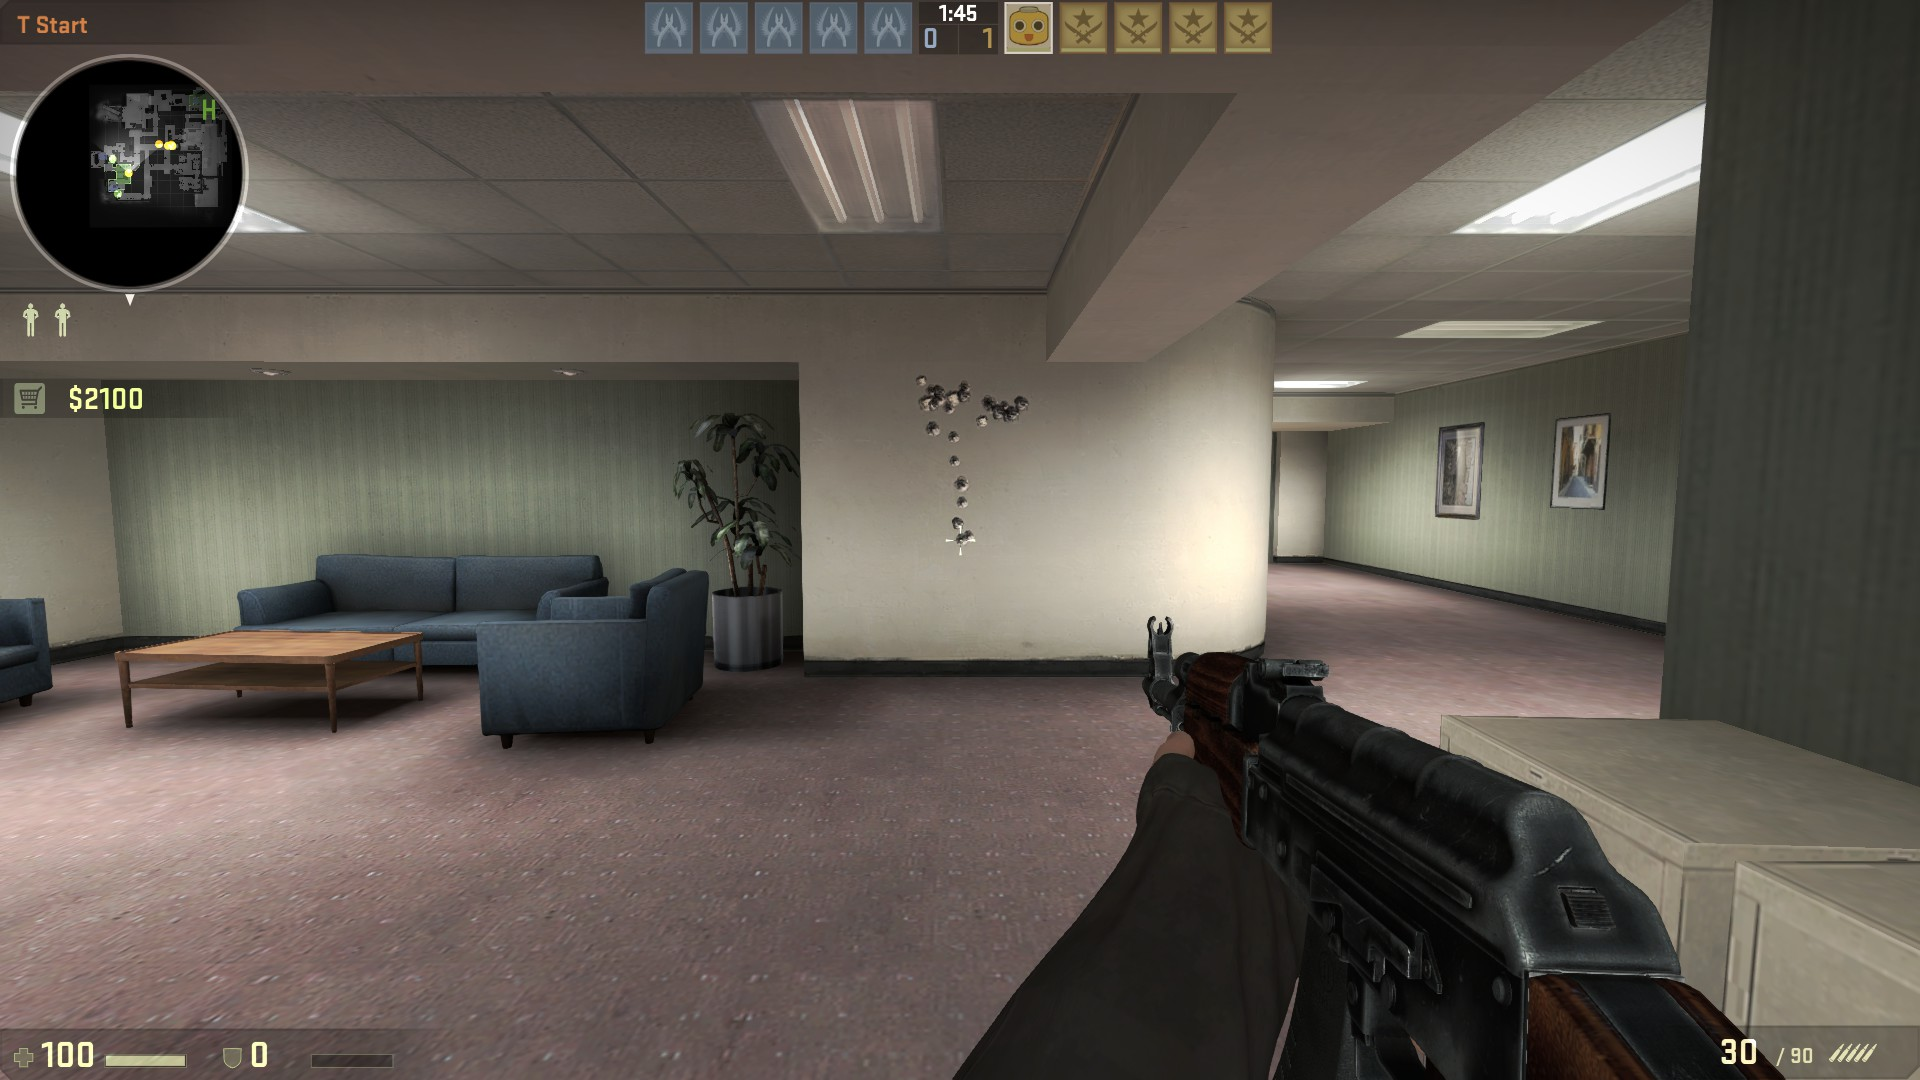
\includegraphics[width=15cm]{img/spraypattern-example}
\caption{Een spray pattern}
\end{figure}  

Het is dus mogelijk om dit tegen te gaan door in omgekeerde richting dit tegen te gaan door de spray te controleren. Dit is een van de cheats die vaak bij aimhacks voorkomt. Zodra de gebruiker begint te schieten worden muisbewegingen gesimuleerd aan de hand van welk wapen ze precies vast hebben. Dan moet de gebruiker wel nog zelf de persoon zien te volgen natuurlijk. En dat is waar de echte aimhacks te pas komen.
\\

De 2e vorm die vaker gebruikt wordt dan bovenstaande is iets moeilijker. Deze zal voor de speler mikken op een vijand en dan nog wel liefst op het hoofd. Hoewel deze moeilijker te maken is vanuit het programmeeraspect. Net zoals voorgaande cheats wordt ook dit in assembly geschreven. Een interessante reeks video's zijn deze van \cite{basicaimbottutorial}. Dit is een forum waarin de basis voor het maken wordt getoond voor het maken van een hack of cheat. In onderstaande afbeelding kan je duidelijk zien dat er gewerkt wordt met de geheugen adressen van het systeem. 

\begin{figure}
\centering
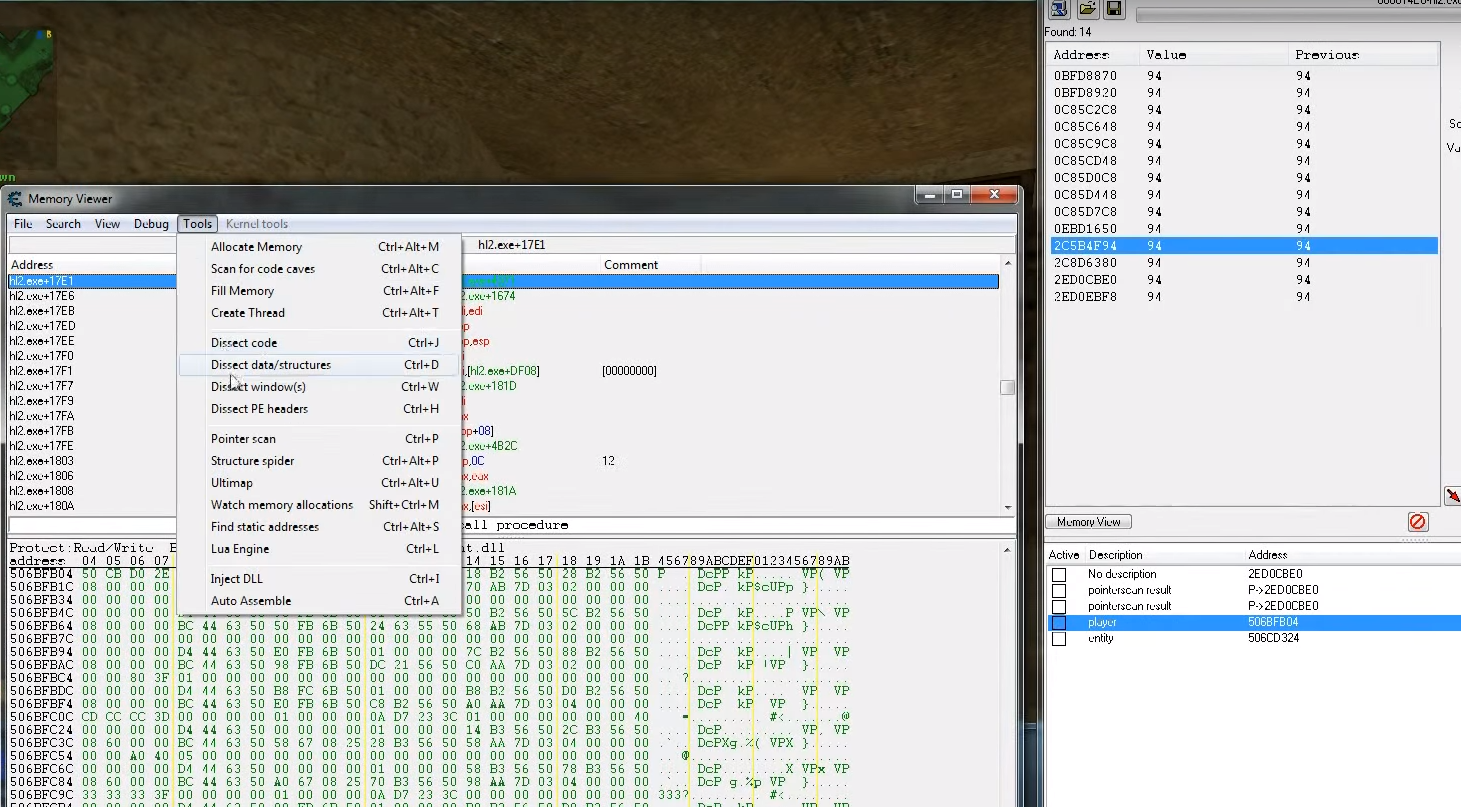
\includegraphics[width=15cm]{img/aimhack-code-example}
\caption{Een voorbeeld van de gebruikte software om de geheugenadressering aan te spreken}
\end{figure}


\chapter{Anti-Cheats}
\label{ch:anticheats}
Het belangrijkste aspect van deze bachelorproef is het tegengaan van het valsspelen. Dit is waar we nu op in zullen gaan. Dit onderdeel wordt opgedeeld in 3 hoofdcategorieën. Eerst de software tools die op de gameserver draaien. Ten tweede heb je dan ook iets nieuw en opkomend: de anti-cheat hardware. Als laatste hebben we nog de sociale of crowd-sourced anti-cheats.

\section{Software}
\label{sec:antisoftware}
Als eerste zullen we even de software overlopen. Dit is de meest voorkomende oplossing en heeft dus ook een waaier aan oplossingen. Omdat het belangrijk is dat anti-cheat software mee is met de laatste vernieuwingen is er hoofdzakelijk geconcentreerd op software die nog altijd actief in development is of lijkt. 

\subsection{VAC: Valve Anti-Cheat}
\label{sec:vac}
De grootste en meest bekende software is de Valve Anti-Cheat software. Dit komt standaard bij iedere installatie van de game en ook iedere server runt dit standaard wanneer deze opgestart wordt. \citep{VAC}Omdat iedere speler deze software staan heeft is dit ook de software die de meeste gebruikers pakt absoluut. In totaal zijn bijna een vier miljoen bans uitgedeeld.
\citep{steamdb}
\\

Hoewel dit heel doeltreffend is kan er toch nog veel beter gewerkt worden aan deze software. In 2014 kwam er een schandaal naar buiten waarbij 3 professionele spelers langere tijd gecheat hadden zonder dat dit gemerkt werd door het Valve Anti-Cheat systeem. Tot een plots moment dan toch, daarna werden deze plots gevangen door VAC en was er heel veel ophef hier rond. Daarna was de vraag die iedereen stelde: wie is de volgende. Er werd een heksenjacht georganiseerd op alle andere professionele spelers. Er was lange tijd twijfel of iedereen wel volledig zelf en eerlijk speelden. Hoewel de gemoederen gestilt zijn is er toch vaak nog sprake over twijfel die onder de kijkers speelt. \citep{pcgamerhackingscandal}
\\

Dus als serveradministrator wordt er vaak gekozen voor een third party tool die dit moet tegengaan. Deze zijn vaak nog iets beter en vaker geüpdate. 


\subsection{Sourcemod}
\label{sec:sourcemod}
Een van de belangrijkste tools die nodig is om geavanceerde wijzigingen door te voeren op een gameserver met de Source engine (de game engine van Valve) zijn pluginsen meer bepaald Sourcemod. Deze biedt nog veel meer functionaliteit aan dan anders mogelijk zou zijn. Er zijn dan ook enkele software pakketten die deze gebruiken om hun functionaliteit doeltreffender te maken. 
\\

Sourcemod is heel eenvoudig zelf te installeren. Men download de benodigde files plaatst deze via FTP op de gameserver in de juiste map en herstart de gameserver. Nadien kun je via commando's nagaan of dit correct werkt. Eenmaal dit correct is ingesteld is het eenvoudig om anti-cheats toe te voegen en of verwijderen. 
%https://wiki.alliedmods.net/Installing_sourcemod

\subsection{SMAC: Sourcemod Anti-Cheat}
\label{sec:smac}


\subsection{Easy Anti-Cheat}
\label{sec:easy}

\subsection{Fairfight}
\label{sec:fairfight}


\section{Hardware}
\label{sec:antihardware}
Iets wat sinds 2014 aangekondigd is, is de Game:ref. Dit is een klein doosje die binnenin een arduino bordje bevat. Wat doet dit juist? Je sluit dit apparaatje aan op je computer en op het internet. Daarna sluit je op het apparaatje je muis aan. Deze heeft het signaal van de muis door aan de computer dus een speler zal er niets van merken. 
Het apparaatje vergelijkt dan via de gameserver (daarom de internetconnectie) of wat de persoon input via zijn muis wel gelijk is aan wat de server doorkreeg. Als dit niet zo is kunnen we concluderen dat er iets gebeurt tussen de muis en de gameserver wat dus duidt op een cheat. 
\\

Het concept zit heel goed in elkaar en zou specifiek aimhacks tegengaan (wallhacks kun je hier niet mee tegenhouden). Het enige probleem hiermee is dat niet iedereen zoiets zal aankopen, laat staan als deze wel zou cheaten, dan ga je echt jezelf niet aangeven. Het lijkt dan ook meer een product gericht op evenorganisers of organisaties. 
\\

De campagne ging van start vorig jaar in april op Kickstarter maar is vrij snel gefaald en weer offline gehaald. Uit een post van de maker op de facebook pagina blijkt wel nog dat dit product in ontwikkeling is dus het kan in de toekomst zeker een interessant product zijn om mensen te controleren die meedoen aan een evenement zoals de professionele spelers.
\citep{gameref} 
\\

Hoewel hier niet mee getest kan worden is dit zeker iets dat wel in overweging moet genomen worden voor toekomstige onderzoeken. Het is iets volledig nieuw en als het concept werkt kan het veelbelovende resultaten halen.

\begin{figure}
\centering
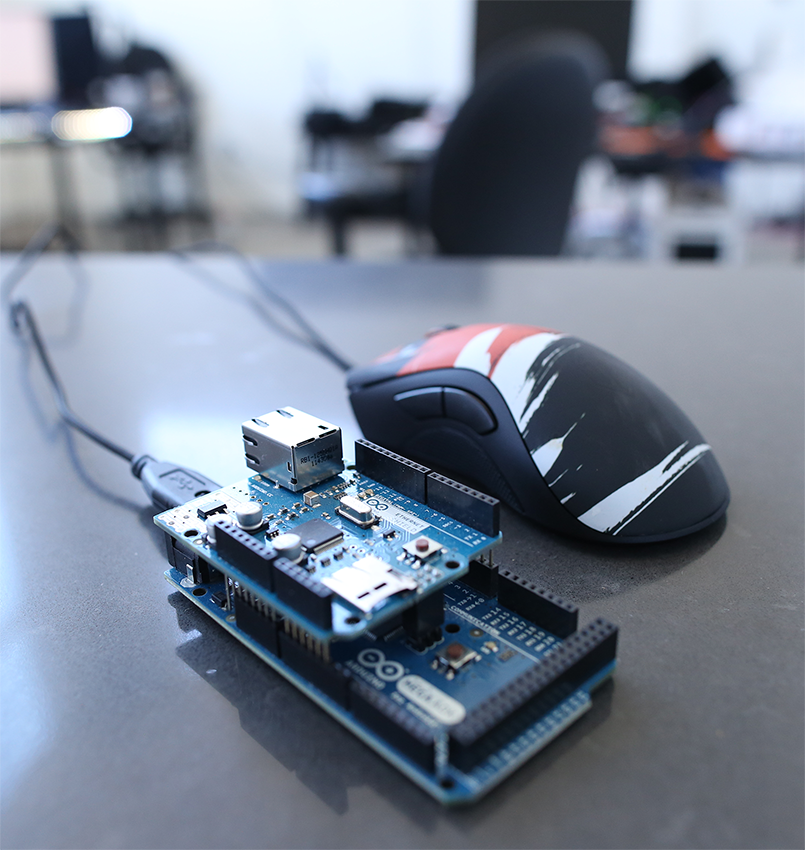
\includegraphics[width=7cm]{img/game-ref1}
\caption{De Game:ref}
\end{figure}



\section{Sociale of Crowd-Sourced}
\label{sec:sociale}
Een van de laatste manieren om aan anti-cheating te doen is via Sociale anti-cheats of ook wel ''Crowd-Sourced''. Dit zijn systemen die gebruikers laat kijken naar verdachte personen en hen laat beslissen of deze al dan niet valsspelen. 
\\

Hiermee zijn wel 3 problemen:
\begin{enumerate}  
\item Eerst en vooral: hoe beslis je wie verdacht is en wie niet. Controleer je iedereen of laat je enkel aangeduide spelers gecontroleerd worden.
\item Ten tweede: wie laat je deze bekijken? Kan iedereen dit of zijn er toch vereisten zodat niet jan en alleman iemand kan veroordelen tot valsspelen. Want wat we ten zeertste willen vermijden zijn mensen die onrechtvaardig verbannen worden.
\item Als derde moeten we ook rekening houden met wanneer je beslist iemand te verbannen van je gameservers. Doen we dit wanneer er een iemand zegt dat deze valsspeelt op basis van 1 kijker? Of laten we meerdere mensen kijken en kijken we hoeveel procent van deze zegt dat de verdachte valsspeelt?
\item En als laatste: Hoe maak je dat mensen dit blijven doen en dit geen vergeten functie wordt? Geef je er iets voor in ruil of hoe houdt je mensen aangetrokken tot de functie.
\end{enumerate}

Dit wordt standaard wel al gedaan bij de laatste versie van Counter-Strike. Deze optie noemt ''Overwatch'' in het spel.
Hoe zij dit beschrijven is als volgt:"The Overwatch lets the CS:GO community regulate itself by allowing qualified and experienced members of the community (‘investigators‘) to review reports of disruptive behavior, determine whether those reports are valid, and apply temporary bans if appropriate." \citep{overwatch}
\\

Hoe werkt dit nu precies? Mensen van een bepaalde rank binnen het spel en die een bepaald aantal spellen al gespeeld hebben krijgen toegang tot de functie. Eenmaal je dit hebt komt er in het start menu een knop waar je een ''Case kan reviewen''. Dit download dan een video bestand waar alle namen van spelers zijn uitgewist. De verdachte noemt ''The Suspect'' en je krijgt een videofragment te zien van een 10 tal rondes. Hierna sluit de video af en krijg je per cheat categorie de optie om te kiezen of jij denkt of deze valsspeelt of niet. Deze case komt ook bij andere spelers terecht, wanneer een bepaald aantal bevestigd (het is onbekend hoeveel precies of procentueel) dan wordt ''The Suspect'' verbannen. Ze proberen je dit te doen aanhouden door je een melding te geven wanneer er iemand verbannen wordt die jij veroordeeld hebt. Op deze manier weten spelers dat ze de game zelf zo van cheaters proper houden en moet dit hen de neiging geven om dit vaker te doen.
\\

De beslissing wie verdacht is wordt genomen aan de hand van de spelers zelf. Als je een officiële match speelt kan je iemand raporteren voor verdacht gedrag. Wanneer een bepaald aantal spelers dit doet komt deze terecht tussen de Overwatch cases.

\begin{figure}
\centering
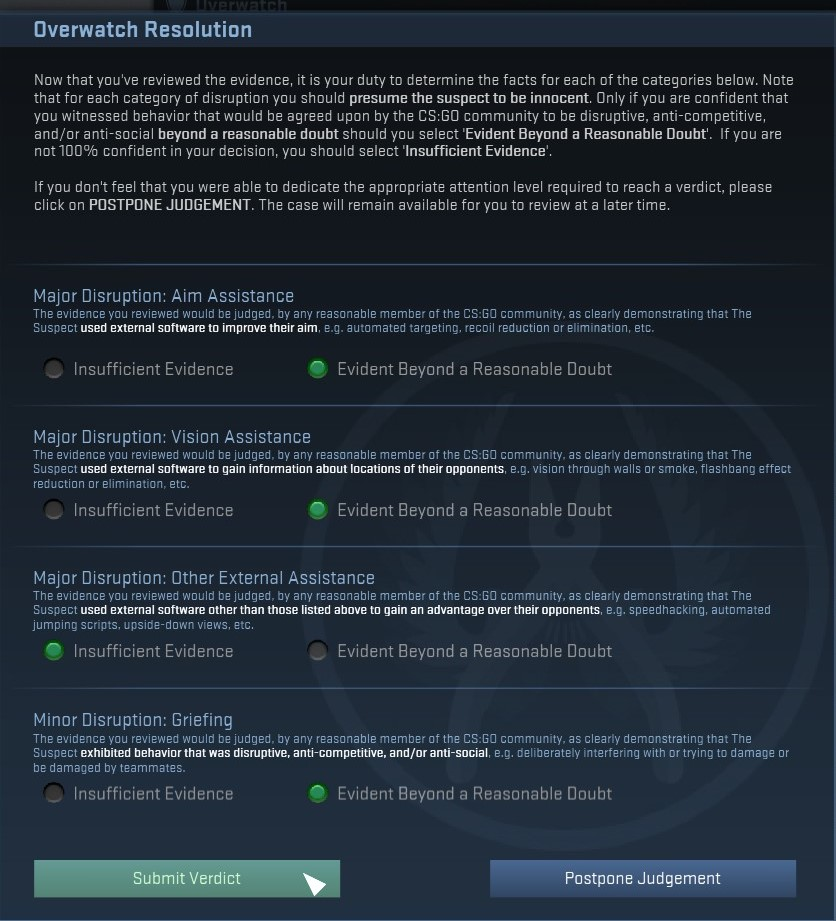
\includegraphics[width=7cm]{img/overwatch-example}
\caption{Een voorbeeld van de opties na het bekijken van een Overwatch video}
\end{figure}


\chapter{De Test}
\label{ch:test}

WIP

\chapter{Interview}
\label{ch:interview}
WIP


\chapter{Conclusie}
\label{ch:conclusie}

% TODO: Trek een duidelijke conclusie, in de vorm van een antwoord op de
% onderzoeksvra(a)g(en). Reflecteer kritisch over het resultaat. Zijn er
% zaken die nog niet duidelijk zijn? Heeft het ondezoek geleid tot nieuwe
% vragen die uitnodigen tot verder onderzoek?



\bibliographystyle{apa}
\bibliography{tin-bachproef}

%%---------- Back matter -------------------------------------------------

\listoffigures
\listoftables

\end{document}
